\documentclass[a4paper]{scrartcl}

%\usepackage{showframe}
\usepackage[margin=2cm,footskip=.7cm]{geometry}
\usepackage{enumitem}
% \usepackage{fourier}
\usepackage{xcolor}
% \usepackage{abkuerzungen}
\usepackage{hyperref}
\usepackage{amsmath}
\usepackage{../../ISASmacros/isasmathmacros}

\usepackage{pdfpages}


\newcommand{\sA}{\ensuremath{\mathsf{A}}}
\newcommand{\sAB}{\ensuremath{\mathsf{AB}}}
\newcommand{\sB}{\ensuremath{\mathsf{B}}}
\newcommand{\sBA}{\ensuremath{\mathsf{BA}}}
\newcommand{\sC}{\ensuremath{\mathsf{C}}}

\newcommand{\cest}{\ensuremath{\cvec{\gamma}}}
\newcommand{\cerest}{\ensuremath{\ervec{\gamma}}}
\newcommand{\cmat}{\ensuremath{\mat{\Gamma}}}
\newcommand{\tmat}{\ensuremath{\widetilde{\mat{\Gamma}}}}

\newcommand{\gainA}{\ensuremath{\mat{K}}}
\newcommand{\gainB}{\ensuremath{\mat{L}}}

% \newcommand{\fus}{\ensuremath{\op{fus}}}

% \newcommand{\CI}{\op{CI}\xspace}
% \newcommand{\EI}{\op{EI}\xspace}
% \newcommand{\ICI}{\op{ICI}\xspace}
% \newcommand{\BC}{\op{B\!/\!C}\xspace}
% \newcommand{\ind}{\op{s}\xspace}
\newcommand{\ind}{\op{in}\xspace}
\newcommand{\opt}{\cmat}


\newcommand{\excmat}{\ensuremath{\mat{\Gamma}'}}
\newcommand{\excest}{\ensuremath{\cest'}}
% \newcommand{\exoptmat}{\ensuremath{\mat{C}_{\excmat}}}
\newcommand{\exoptmat}{\ensuremath{\mat{C}'_\EI}}

%\RequirePackage[mathscr]{euscript}
%\RequirePackage{bbding}
%\RequirePackage{scalefnt}
%\RequirePackage{mathtools}
% This was enabled but makes the text look ugly
%\RequirePackage[T1]{fontenc}


%%% COLOR DEFINITIONS

% KIT Colors
\definecolor{kitgreenex}{RGB}{0,152,131}
\definecolor{kitblueex}{RGB}{52,115,186}
\definecolor{kitmaygreen}{RGB}{119,184,38}
\definecolor{kityellow}{RGB}{255,228,0}
\definecolor{kitorange}{RGB}{247,154,0}
\definecolor{kitbrown}{RGB}{182,130,28}
\definecolor{kitred}{RGB}{187,25,23}
\definecolor{kitpurple}{RGB}{190,0,126}
\definecolor{kitcyanblue}{RGB}{0,167,227}
% Own Definitions
\definecolor{grey}{RGB}{150,150,150}


\definecolor{nblue}{RGB}{54,95,145}

%%% FONTS
%\setkomafont{pageheadfoot}{\small\color{darkgray}}
%\setkomafont{pagefoot}{\normalfont\color{darkgray}}
%\setkomafont{pagenumber}{\color{darkgray}}
%\setkomafont{captionlabel}{\small\bfseries\color{darkgray}}
\setkomafont{disposition}{\bfseries}
\setkomafont{section}{\normalfont\large\bfseries}
\setkomafont{subsection}{\normalfont\bfseries}
\setkomafont{author}{\normalfont}
\setkomafont{date}{\normalfont}


%%% PARAGRAPH LAYOUT
\setlength{\parindent}{0mm}
\setlength{\parskip}{6pt}


%%% REBUTTAL COMMANDS
\newenvironment{rebuttal}{\begin{enumerate}[label={\color{grey}\thesection.\arabic{enumi}},leftmargin=0pt,ref=\thesection.\arabic{enumi}]}{\end{enumerate}}
\newcommand{\reviewtext}[1]{{\color{nblue} #1}}
\newcommand{\papertext}[1]{\emph{``#1''}}

%%% HYPERREF SETUP
\hypersetup{
        colorlinks = true,
        linkcolor = kitgreenex
}

%%%%%%%%%%%%%%%%%%%%%%%%%%%%%%%%%%%%%%%%%%%%%%%%%%%%%%%%%%%%%%%%%%%%%%%%

\title{\boldmath Cryptographically Privileged State Estimation With Gaussian Keystreams}
\subtitle{Response to Reviewers' Comments - Submission L-CSS 21-0154}
\author{Marko Ristic\and Benjamin Noack\and Uwe D. Hanebeck}

%       .d8888b.  888                     888
%      d88P  Y88b 888                     888
%      Y88b.      888                     888
%       "Y888b.   888888  8888b.  888d888 888888
%          "Y88b. 888        "88b 888P"   888
%            "888 888    .d888888 888     888
%      Y88b  d88P Y88b.  888  888 888     Y88b.
%       "Y8888P"   "Y888 "Y888888 888      "Y888

\begin{document}

\maketitle

Dear Dr. Ji-Feng Zhang,\\
Dear Reviewers,

We would like to thank you all for your responses and agreement on accepting our manuscript. As specified in the Author's Checklist, we list the changes made to the accepted manuscript here. The changes consist of switching to the final version template and minor wording and spelling changes. Throughout this response, reviewers' comments are in \reviewtext{blue}. 

Sincerely,\\
Marko Ristic, Benjamin Noack, and Uwe D. Hanebeck

%      8888888888     888 d8b 888
%      888            888 Y8P 888
%      888            888     888
%      8888888    .d88888 888 888888 .d88b.  888d888
%      888       d88" 888 888 888   d88""88b 888P"
%      888       888  888 888 888   888  888 888
%      888       Y88b 888 888 Y88b. Y88..88P 888
%      8888888888 "Y88888 888  "Y888 "Y88P"  888

\section*{Response to the Editor's Report}
\def\thesection{E}
\begin{rebuttal} %\setcounter{enumi}{-1}
\item \reviewtext{All the Reviewers are fine with the revised version. Accordingly, I am glad to recommend the paper publication. 

One reviewer pointed out a possible small typo in a reference. I have checked that: the reference given by the authors is correct. I guess the reviewer found the draft of the book in http://staff.ustc.edu.cn/\\\~{}mfy/moderncrypto/reading\%20materials/Introduction\_to\_Modern\_Cryptography.pdf which does not correspond exactly with the published version.}

We are happy to hear of your decision, thank you. Regarding the reference, we have left it as it was submitted in the accepted version.

\end{rebuttal}

%      8888888b.                         d888
%      888   Y88b                       d8888
%      888    888                         888
%      888   d88P .d88b.  888  888        888
%      8888888P" d8P  Y8b 888  888        888
%      888 T88b  88888888 Y88  88P        888
%      888  T88b Y8b.      Y8bd8P         888
%      888   T88b "Y8888    Y88P        8888888

\section*{Response to the Comments of Reviewer 1 (46379)}
\def\thesection{R1}
\begin{rebuttal}
\item \reviewtext{The authors have answered all my earlier concerns.}

We are glad to hear this, thank you.

\end{rebuttal}

%      8888888b.                         .d8888b.
%      888   Y88b                       d88P  Y88b
%      888    888                              888
%      888   d88P .d88b.  888  888           .d88P
%      8888888P" d8P  Y8b 888  888       .od888P"
%      888 T88b  88888888 Y88  88P      d88P"
%      888  T88b Y8b.      Y8bd8P       888"
%      888   T88b "Y8888    Y88P        888888888

\section*{Response to the Comments of Reviewer 2 (46381)}
\def\thesection{R2}
\begin{rebuttal}
\item \reviewtext{The authors have addressed my comments}

We are happy we could address them all, thank you.

\end{rebuttal}

%      8888888b.                         .d8888b.
%      888   Y88b                       d88P  Y88b
%      888    888                            .d88P
%      888   d88P .d88b.  888  888          8888"
%      8888888P" d8P  Y8b 888  888           "Y8b.
%      888 T88b  88888888 Y88  88P      888    888
%      888  T88b Y8b.      Y8bd8P       Y88b  d88P
%      888   T88b "Y8888    Y88P         "Y8888P"

\section*{Response to the Comments of Reviewer 3 (44309)}
\def\thesection{R3}
\begin{rebuttal}
\item \reviewtext{The reviewer only have the following one more suggestion.

1.Could the author explain more about the negligible function \textbackslash eta in Definition 2.3. and make a definition of this function in this paper? The reviewer cannot find the definition 3.4. in ref [8] which may be a different version.}

We're sorry to hear that the reference was not easier to find. The editor has indicated that the reference was correct and differs from the book draft that can be found online, so we have left it unchanged. We're glad we could address your remaining suggestions.

\end{rebuttal}

%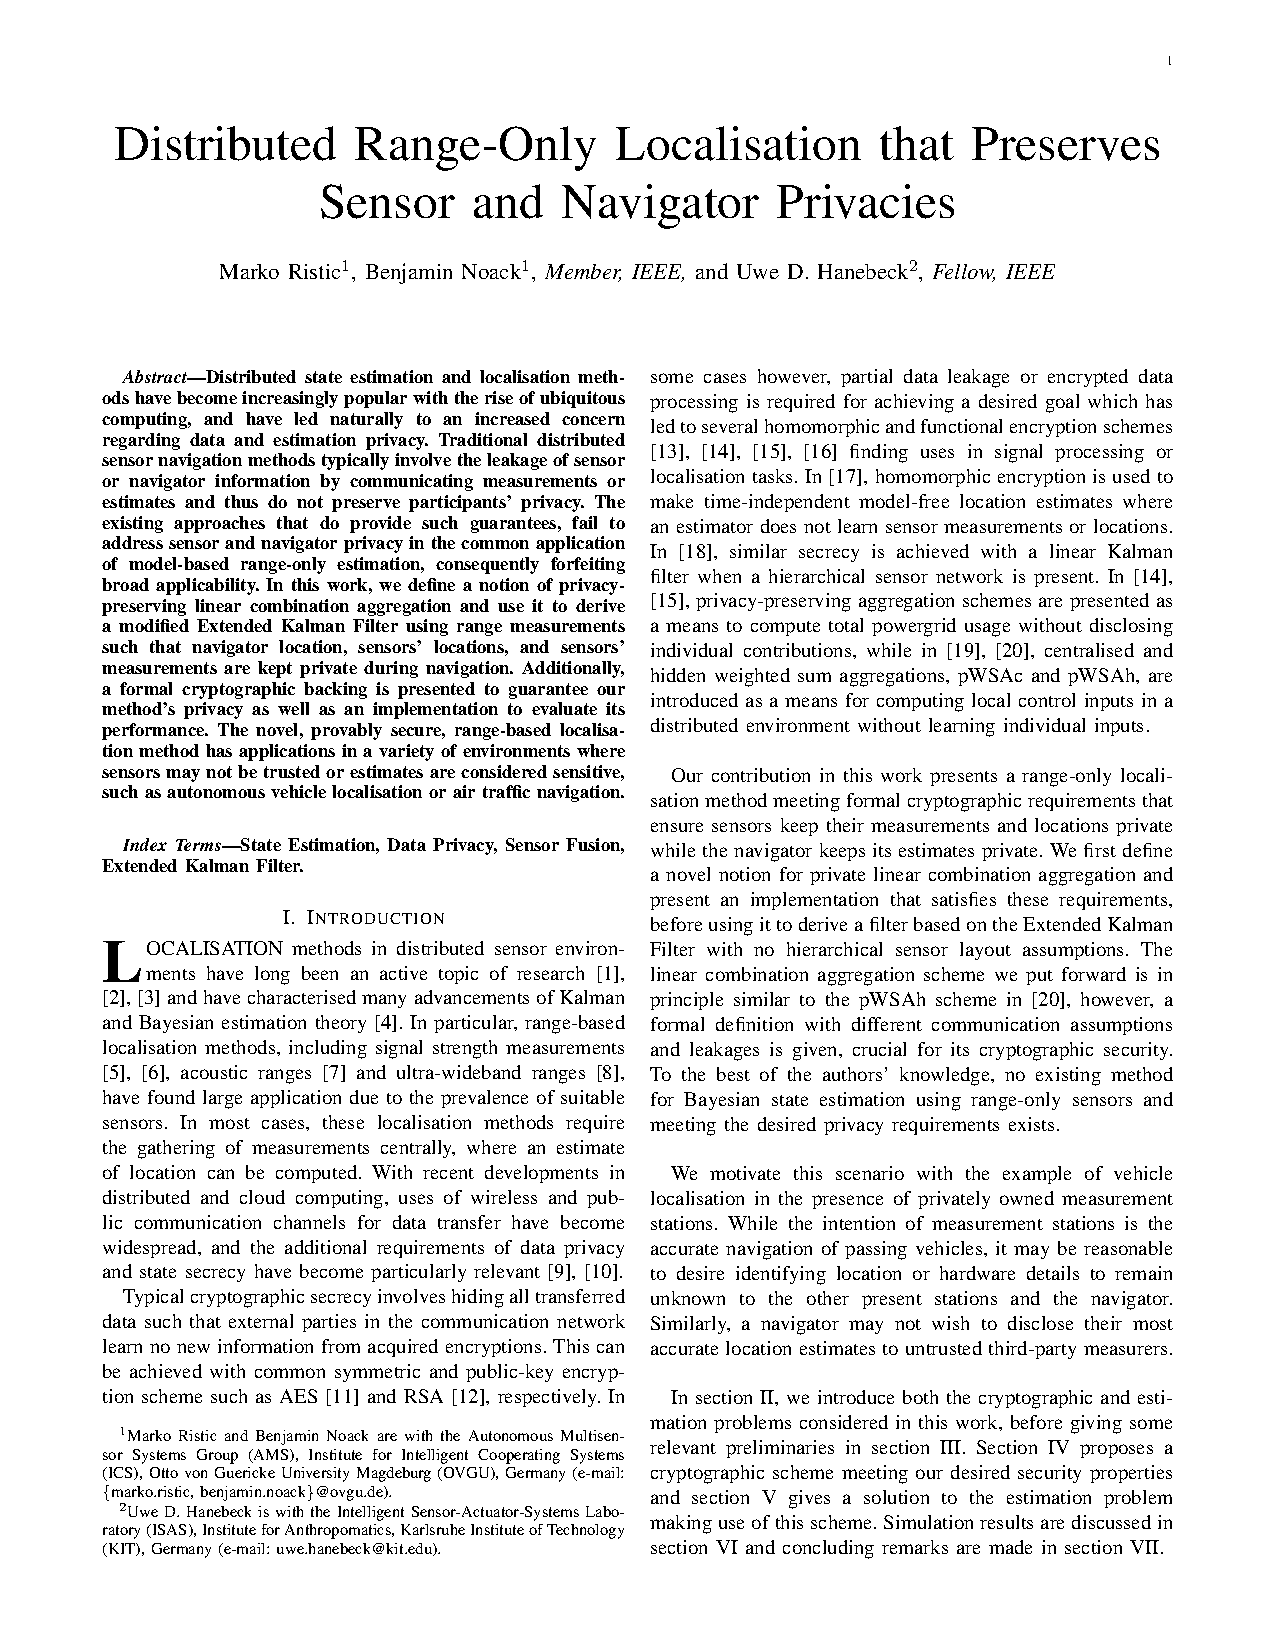
\includepdf[pages=-]{diff}

\end{document}